% Generated by code/ch01_tomography_scaling.py -- do not edit by hand.
\definecolor{qocA}{rgb}{0.00,0.45,0.70}
\definecolor{qocB}{rgb}{0.90,0.60,0.00}
\definecolor{qocC}{rgb}{0.00,0.62,0.45}
\definecolor{qocD}{rgb}{0.80,0.40,0.00}
\definecolor{qocE}{rgb}{0.80,0.60,0.70}
\definecolor{qocF}{rgb}{0.35,0.70,0.90}
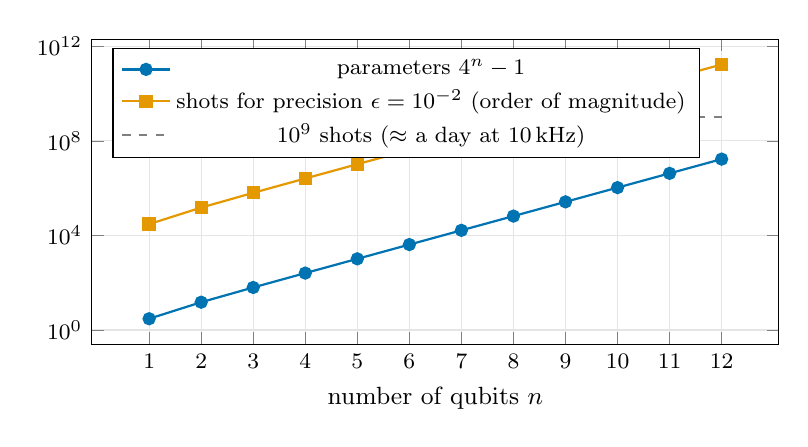
\begin{tikzpicture}[]
\begin{axis}[width=0.85\linewidth, height=0.45\linewidth, xlabel={number of qubits $n$}, ylabel={}, legend pos=north west, legend style={font=\footnotesize}, tick label style={font=\footnotesize}, label style={font=\small}, grid=major, grid style={gray!20}, ymode=log, xtick=data]
\addplot[thick, qocA, mark=*] coordinates {(1,3) (2,15) (3,63) (4,255) (5,1023) (6,4095) (7,16383) (8,65535) (9,2.6214e+05) (10,1.0486e+06) (11,4.1943e+06) (12,1.6777e+07)};
\addplot[thick, qocB, mark=square*] coordinates {(1,30000) (2,1.5e+05) (3,6.3e+05) (4,2.55e+06) (5,1.023e+07) (6,4.095e+07) (7,1.6383e+08) (8,6.5535e+08) (9,2.6214e+09) (10,1.0486e+10) (11,4.1943e+10) (12,1.6777e+11)};
\addplot[thick, qocC, gray, dashed] coordinates {(1,1e+09) (2,1e+09) (3,1e+09) (4,1e+09) (5,1e+09) (6,1e+09) (7,1e+09) (8,1e+09) (9,1e+09) (10,1e+09) (11,1e+09) (12,1e+09)};
\legend{{parameters $4^n-1$}, {shots for precision $\epsilon=10^{-2}$ (order of magnitude)}, {$10^{9}$ shots ($\approx$ a day at $10\,$kHz)}}
\end{axis}
\end{tikzpicture}
